\chapter{Relazione tirocinio}
\label{cha:conclusioni}


In questo capitolo viene esposto un resoconto del tirocinio avvenuto tra i mesi di aprile e maggio 2019 presso il Liceo Galileo Galilei (Trento), il liceo Leonardo Da Vinci (Trento) e l’istituto tecnico tecnologico Buonarroti-Pozzo (Trento). L’attività è stata strutturata in due parti: una parte teorica di lezione interattiva e una parte laboratoriale in cui i ragazzi svolgevano degli esercizi. Lo scopo del tirocinio è stato quello di proporre un modo diverso di visualizzare ed utilizzare l’informatica presso gli istituti superiori, seguendo i principi del modello Computational STEAM (vedi Capitolo 1). L’argomento trattato, i protocolli epidemici (vedi Capitolo 2), è stato scelto perché adatto a far comprendere come modelli e algoritmi studiati in altri campi (la biologia e la matematica) possano essere adattati ed utilizzati con efficacia in ambito informatico (nello specifico la comunicazione in sistemi distribuiti).
\section{Contesto e organizzazione del corso}
Essendo tre studenti abbiamo organizzato questa esperienza di tironcio nel seguente modo: ognuno ha portato un argomento diverso, ma con le stesse modalita' di presentazione (seguendo i principi di Computatonal STEAM) in tre classi per un totale di 9 classi.
Abbiamo presentato il corso tra aprile e maggio presso i seguenti istituti superiori: liceo Scientifico Galileo Galilei di Trento, liceo Scientifico Leonardo Da Vinci di Trento e istituto tecnico e tecnologico Buonarroti-Pozzo. Abbiamo scelto questo periodo in quanto più adatto sia per i ragazzi che per gli insegnanti ordinari. Ci siamo concentrati sul liceo scientifico, in quanto il percorso di studi Computational STEAM è indirizzato a questa tipologia di scuola, ma abbiamo deciso di provare a portare l’esperienza anche in un istituto tecnico, per cercare di capire quali possono essere le differenze riguardo la preparazione dei ragazzi, in modo da adattare le lezioni al meglio. Abbiamo strutturato le lezioni nel seguente modo: un’ora per l’introduzione, e le restanti 6 ore per il contenuto del corso in sé. La lezione introduttiva e l’ultima sono state utilizzate anche per compilare un questionario introduttivo ed un conclusivo (entrambi anonimi), i cui risultati verranno utilizzati come supporto alla stesura di questo capitolo. È stata utilizzata l’applicazione Moduli Google. Abbiamo raccolto le risposte di 164 ragazzi per il questionario iniziale, 161 per quello finale (- risposte da rimuovere). Questi sono i dati aggrgati per tutte le classi. Utilizziamo i dati aggragati per la parte  di contesto, mentre per la parte "tecnica" li suddividiamo in base al corso frequentato (alcune domande sono specifiche del modulo, come quelle riguardante il feedback riscontrato, il quale puo' variare in base a chi ha presentato il corso).
Le classi a cui sono rivolti sono terze, quarte e quinte, perché gli argomenti trattati risultano più adatti a studenti con conoscenze che vengono fornite a partire dal terzo anno in poi. La scelta delle classi è stata fatta dagli insegnanti di informatica, a cui sono stati proposti i moduli.
\begin{figure}[!h]
    \begin{subfigure}{.5\textwidth}
        \centering
        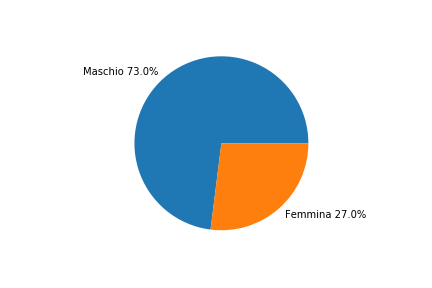
\includegraphics[width=\textwidth]{genere.png}
        \caption{Genere}
        \label{fig:genere}
    \end{subfigure}\hfill
    \begin{subfigure}{.5\textwidth}
        \centering
        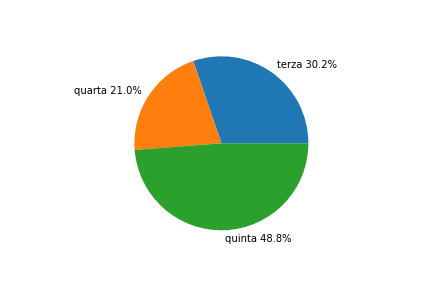
\includegraphics[width=\textwidth]{classi.png}
        \caption{Classi}
        \label{fig:classi}
    \end{subfigure}
    \caption{Caratteristiche del campione} 
\end{figure}
\subsection{Analisi del campione}
Le classi sono prevalente composte da maschi, il che non è affatto sorprendente osservando la composizione nei corsi di studio di informatica ed ingegneria. I ragazzi hanno notato questa differenza numerica, motivandola principalmente con questa affermazione: “l'informatica è preferita dai ragazzi”. Nonostante ciò, la figura dell’informatico è stata descritta in modo abbastanza lontano dai frequenti stereotipi: secondo i dati raccolti molti pensano che un informatico debba essere creativo e abbia grande capacità nel lavorare in gruppo. 

\section{Contenuto e metodo esecutivo} 
Il contenuto del corso è stato esposto utilizzando delle slide per la parte di lezione teorica, mentre per la parte applicativa è stata fornita una cartella condivisa con gli esercizi da svolgere e le loro spiegazioni nel dettaglio (\href{http://www.tinyurl.com/protocolli-epidemici}{http://www.tinyurl.com/protocolli-epidemici}). La parte teorica è stata presentata come lezione interattiva, dando spazio agli studenti di porci delle domande e di rispondere a quesiti da noi proposti. Ad eccezione della prima ora di lezione, tutte le altre hanno avuto una componente pratica, in modo tale che i ragazzi potessero applicare quanto imparato. La difficoltà degli esercizi è via via crescente, sia per la complessità degli algoritmi proposti, sia per un minore aiuto fornito in determinate situazioni (in alcuni casi è stato fornito solamente lo pseudocodice). 
Abbiamo scelto di sviluppare il corso sui protocolli epidemici (vedi Capitolo 2) per diversi motivi: in primo luogo, l’argomento si basa su semplici regole che vengono utilizzate più volte in diversi contesti. I protocolli di gossip possono però essere studiati maggiormente e lasciano spazio anche ad un approfondimento autonomo. Inoltre sono sono un argomento interdisciplinare: vengono utilizzati in reti distribuite per la comunicazione, ma i principi su cui si basano sono studiati in epidemiologia, nell’ambito quindi della diffusione delle epidemie, ma anche dalle scienze sociali, riguardo il fenomeno del gossip. Questa interdisciplinarietà si dimostra adatta all’interno di questa esperienza che vuole portare i principi di Computational STEAM nelle scuole superiori.
Nello specifico abbiamo abbiamo sviluppato il programma del corso nel seguente modo: nella prima lezione, utile come introduzione, abbiamo presentato l’argomento e la sua natura interdisciplinare, il contesto storico, la definizione del problema, le applicazioni reali e i principi di base.
\begin{figure}[!h]
    
    \begin{subfigure}{.5\textwidth}
        \centering
        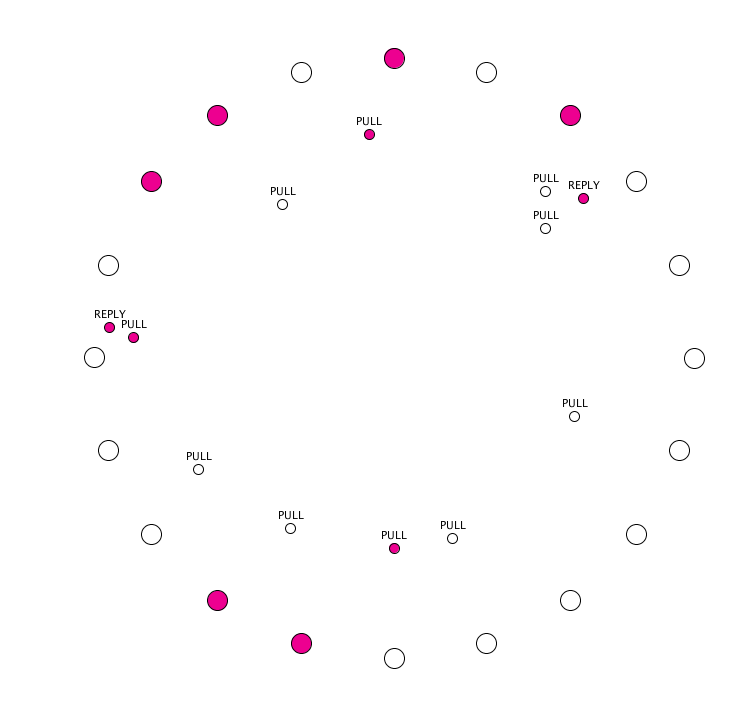
\includegraphics[width=\textwidth]{pull.png}
        \captionsetup{justification=centering}
        \caption{Algoritmo modello SI: pull} 
    \end{subfigure}\hfill
    \begin{subfigure}{.5\textwidth}
        \centering
        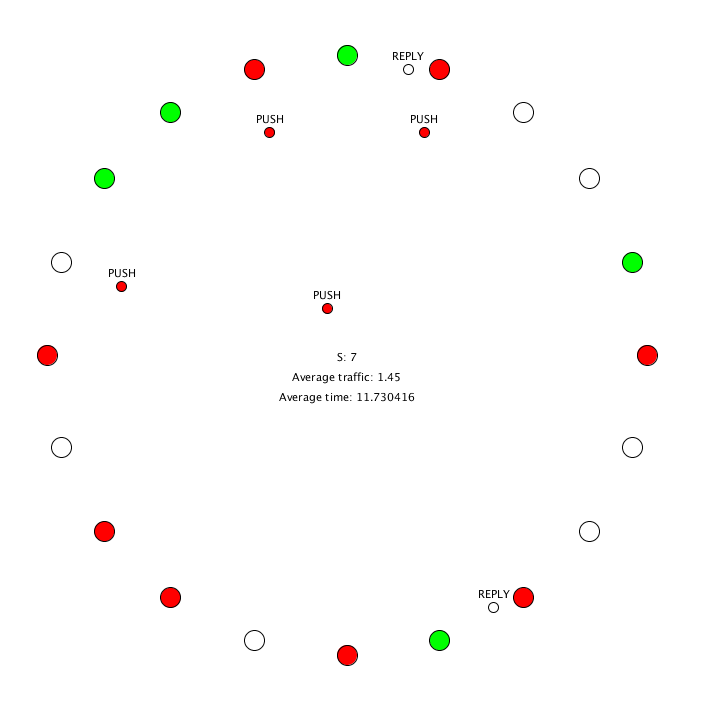
\includegraphics[width=\textwidth]{feedback-counter.png}
        \captionsetup{justification=centering}
        \caption{Algoritmo modello SIR: feedback-counter} 
    \end{subfigure}
    \caption{Esempi di output}
    \label{fig:output}
\end{figure} 
Nelle successive lezioni ci siamo concentrati, dopo aver fatto una breve introduzione sui grafi (utile per alcune definizioni ed assunzioni), sui due modelli SI e SIR presentando gli algoritmi e stili che li utilizzano, lasciando poi spazio ai ragazzi di implementarli su schermo. L’ambiente di sviluppo utilizzato è Processing (\href{https://processing.org}{https://processing.org}), libreria grafica di Java e IDE utile per creare simulazioni e metodi di visualizzazione efficace. Gli studenti si sono occupati di scrivere gli algoritmi, completando il codice fornito oppure interpretando lo pseudo codice (l'output di alcuni esercizi in Figura \ref{fig:output}). Abbiamo fornito una libreria (\href{https://github.com/ainter21/epidemic}{https://github.com/ainter21/epidemic}), utile sia per alleggerire il carico di lavoro, sia per nascondere alcune componenti troppo complesse, come la parte di visualizzazione (lo scopo degli esercizi è quello di implementare l’algoritmo, mentre la parte di visualizzazione è solamente un supporto per rendere più chiari i concetti).
Abbiamo fornito la documentazione utile per completare gli esercizi, con la spiegazione dei metodi e degli attributi. Il loro obiettivo è stato quindi utilizzare la libreria fornita (con metodi molto simili a quelli utilizzati nell' pseudocodice), affinché gli algoritmi proposti funzionassero. La lista degli esercizi proposti già completati è scaricabile qui (\href{https://github.com/ainter21/epidemic-protocols}{https://github.com/ainter21/epidemic-protocols}).
Abbiamo svolto le attività in laboratori forniti di PC e da proiettore, in modo da proiettare i lucidi e permettere ai ragazzi di lavorare in autonomia o a gruppi. L'idea iniziale era di formare dei gruppi di lavoro per poter collaborare e sviluppare abilità di problem solving e lavoro di squadra. Questa soluzione si  è rivelata di difficile attuazione in quanto i ragazzi possiedono un account personale non condivisibile e se alcuni studenti rimanevano assenti, si rischiava di non ppoter accedere al lavoro iniziato la volta precedente. Abbiamo comunque fatto il possibile per invogliarli a lavorare in gruppo.
\section{Analisi dei risultati}

\begin{figure}[h]
    
    \begin{subfigure}{.5\textwidth}
        \centering
        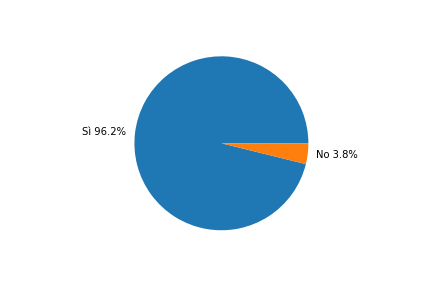
\includegraphics[width=\textwidth]{aspettative.png}
        \captionsetup{justification=centering}
        \caption{Ritieni che siano state \\ soddisfatte le tue aspettative?} 
    \end{subfigure}\hfill
    \begin{subfigure}{.5\textwidth}
        \centering
        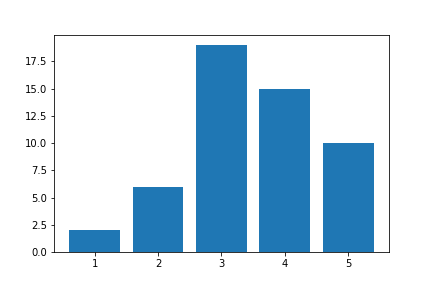
\includegraphics[width=\textwidth]{conoscenze.png}
        \captionsetup{justification=centering}
        \caption{Quanto il corso era adatto  \\ al tuo livello di conoscenze?} 
    \end{subfigure}
    \caption{Risultati}
\end{figure} 

Dopo le sette ore previste, abbiamo chiesto di compilare un questionario di valutazione delle attività svolte.  I dati analizzati in questa sezione non sono i dati aggregati: abbiamo considerato 60 risposte per il questionario iniziale, e 52 per il questionario finale, ovvero quelle riguardanti il modulo "protocolli epidemici".
 I risultati sono positivi, la maggior parte degli studenti dice di essere rimasto soddisfatto. Gli argomenti trattati erano una novità per la maggior parte dei ragazzi, ed alcuni hanno riferito di voler approfondire l'argomento (sia per quanto riguarda l'utilizzo di Processing, sia per i protocolli epidemici, sia per la diffusione delle epidemie).